\documentclass[a4paper,12pt]{article}
\usepackage[pdftex]{graphicx}
\usepackage{tikz}
\usepackage{float}
\usepackage[document]{ragged2e}
\usepackage[utf8]{inputenc}
\usepackage[T1]{fontenc}
\usepackage[spanish,es-tabla]{babel}
\renewcommand{\shorthandsspanish}{}
\usepackage{xurl}
\usepackage{lipsum}
\usepackage{mwe}
\usepackage{multicol}
\usepackage{siunitx}
\usepackage{listings}
\usepackage{circuitikz}

\graphicspath{ {/home/saikkopat/Documents/school/CE/P1/figs/} }

\title{Práctica 1: Uso del óhmetro, voltímetro y amperímetro en mediciones de corriente directa}
\author{González Cárdenas Ángel Aquilez \and Sánchez González Daniel Iván}

\begin{document}

\begin{titlepage}
	\begin{tikzpicture}[overlay, remember picture]
		\path (current page.north east) ++(-0.3,-1.5) node[below left] {
\includegraphics[width=0.35\textwidth]{/home/saikkopat/Documents/LOGOS IPN/EscudoESCOM}};
	\end{tikzpicture}
	\begin{tikzpicture}[overlay, remember picture]
		\path (current page.north west) ++(1.5,-1) node[below right] {
\includegraphics[width=0.2\textwidth]{/home/saikkopat/Documents/LOGOS IPN/logo}};
	\end{tikzpicture}
	\begin{center}
		\vspace{-3cm}
		{\LARGE Instituto Politécnico Nacional\par}
		\vspace{.5cm}
		{\LARGE Escuela Superior de Cómputo\par}
		\vspace{.5cm}
		{\Large Laboratorio de Circuitos Eléctricos\par}
		\vspace{2cm}
		{\large Unidad de aprendizaje:}\\{\Large Circuitos Eléctricos\par}
		\vspace{2cm}
		{\scshape\Huge Práctica 1\par}
		{\itshape\Large Uso del óhmetro, voltímetro y amperímetro en mediciones de corriente directa\par}
		\vfill
		\vspace{.7cm}
		{\Large Grupo: 3CV2\par}
		\vspace{.7cm}
		{\Large Equipo: 5\par}
		\vspace{.7cm}
		{\Large Integrantes:\\González Cárdenas Ángel Aquilez\\Sánchez González Daniel Iván\par}
		\vspace{1cm}
		{\Large Profesor: Vázquez Ortíz Mijaíl\par}
		\vspace{1cm}
		{\large Fecha de realización: 6 de marzo de 2023\par}
		{\large Fecha de entrega: 13 de marzo de 2023\par}
		\vfill
	\end{center}
\end{titlepage} 

\newpage

\tableofcontents

\newpage



\section*{Objetivo}

\textbf{Objetivo}: El alumno comprenderá el manejo adecuado de los instrumentos de medición, por lo que al término de la práctica, deberá estar capacitado para utilizar adecuadamente el óhmetro, voltímetro y amperímetro digitales.\par

El alumno utilizara los siguientes materiales y equipo:
\vspace{.5cm}
\begin{multicols}{2}
\textbf{Equipo}\\
\begin{itemize}
	\item 1 Multímetro digital
	\item 1 Fuente de voltaje variable
	\item 4 puntas banana-caimán
	\item 2 puntas caimán-caimán
\end{itemize}

\columnbreak

\textbf{Material}\\
\begin{itemize}
	\item 1 \textit{Protoboard}
	\item 1 Resistor de 1k \si{\ohm}
	\item 1 Resistor de 560 \si{\ohm}
	\item 1 Resistor de 680 \si{\ohm}
	\item 1 Resistor de 330 \si{\ohm}
	\item Alambres para conexiones
\end{itemize}

\end{multicols}

Notese que todos los resistores deben trabajar a una potencia de $\frac{1}{4}$ de \si{\watt}

\vspace{1cm}

\section{Introducción teórica}

La corriente o el voltaje pueden medirse por medio de amperímetros o voltímetros, la Figura \ref{fig1} muestra dos formas comunes de medidores; uno de los medidores analógico tiene una aguja indicadora que se mueve sobre una escala calibrada cuya deflexión angular depende de la magnitud de la variable que mide. Mientras que el otro es un medidor digital el cual muestra una serie de dígitos en la pantalla, indicando la magnitud de la variable que mide. La Figura \ref{fig2} muestra los símbolos del voltímetro y el amperímetro que se utilizan en los diagramas de circuitos eléctricos.\par

\vspace{.5cm}

\begin{figure}[!h]
\centering
\begin{minipage}{.5\textwidth}
  \centering
	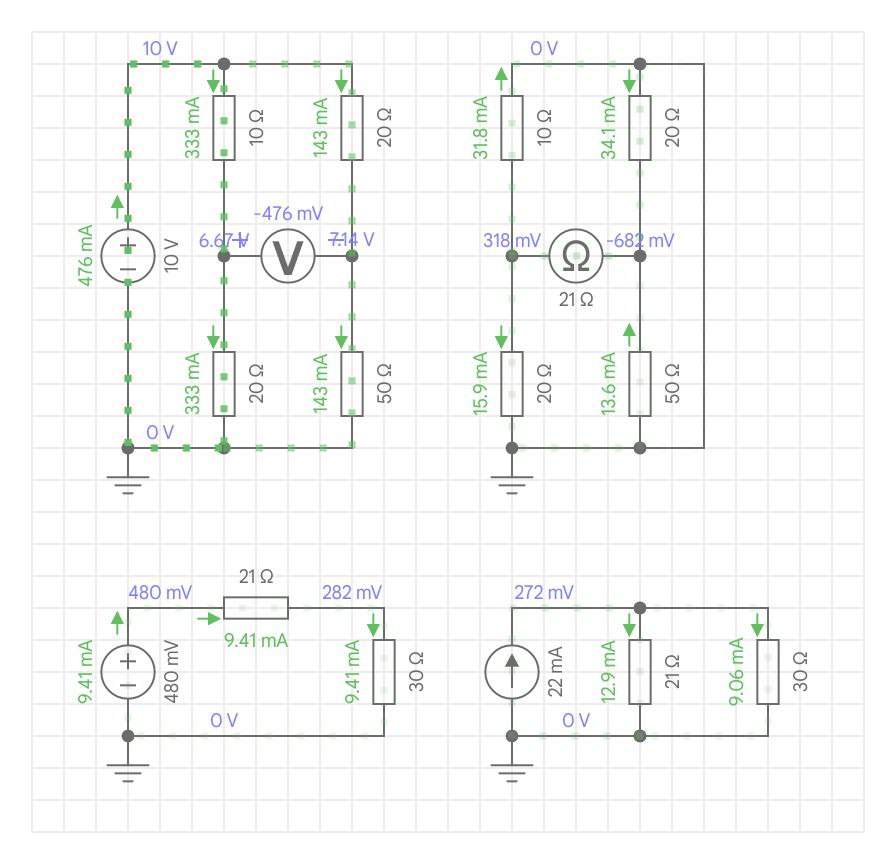
\includegraphics[width=0.5\textwidth]{fig1}
	\label{fig1}
  \caption{Medidores}{a) Analógico, y b) Digital}
\end{minipage}%
\begin{minipage}{.5\textwidth}
  \centering
	\begin{circuitikz} \draw
		(0,0) to[ammeter] (0,4)
		;
	\end{circuitikz}
	\hspace{1cm}
	\begin{circuitikz} \draw
	(0,0) to[voltmeter] (0,4)
	;
	\end{circuitikz}
	\caption{Símbolo de cada medidor}
	\label{fig2}
\end{minipage}
\end{figure}

Para medir la corriente en la rama de un circuito, debe de abrirse esa rama y el amperímetro debe ser insertado de tal manera que quede conectado en serie con el elemento del que se desea conocer su corriente.\\
Se dice que dos elementos están en \textit{serie} si un extremo de uno se une con un extremo del otro, y no existe algún conductor conectado a esa unión. La corriente que circula por esa trayectoria, pasa forzosamente por el medidor de corriente (amperímetro).\par

Para medir el voltaje entre dos puntos, el voltímetro se conecta en \textit{paralelo} con el dispositivo electrónico del que se desea conocer la caída de voltaje. Dos elementos de dos terminales están conectados en paralelo si las terminales de uno están conectadas a las terminales el otro. No importa si en esas uniones hay o no otra conexión. La característica esencial de una conexión en paralelo, que a través de los elementos existe el mismo voltaje.\par

\vspace{1cm}

\section{Desarrollo}
\subsection{Uso del óhmetro}

Sin energizar ningún elemento de circuito, se midió el valor de la resistencia que presenta cada resistor, como se indica en la Figura 3.\par

\vspace{.5cm}

\begin{figure}[!h]
	\centering
	\begin{minipage}{.5\textwidth}
  \centering
  \begin{circuitikz}[american] \draw
		(0,0) to[R=Resistor] (0,3) -- (2,3)
		to[ohmmeter=Óhmetro] (2,0) -- (0,0)	;
	\end{circuitikz}
	\end{minipage}%
	\begin{minipage}{.5\textwidth}
  \centering
	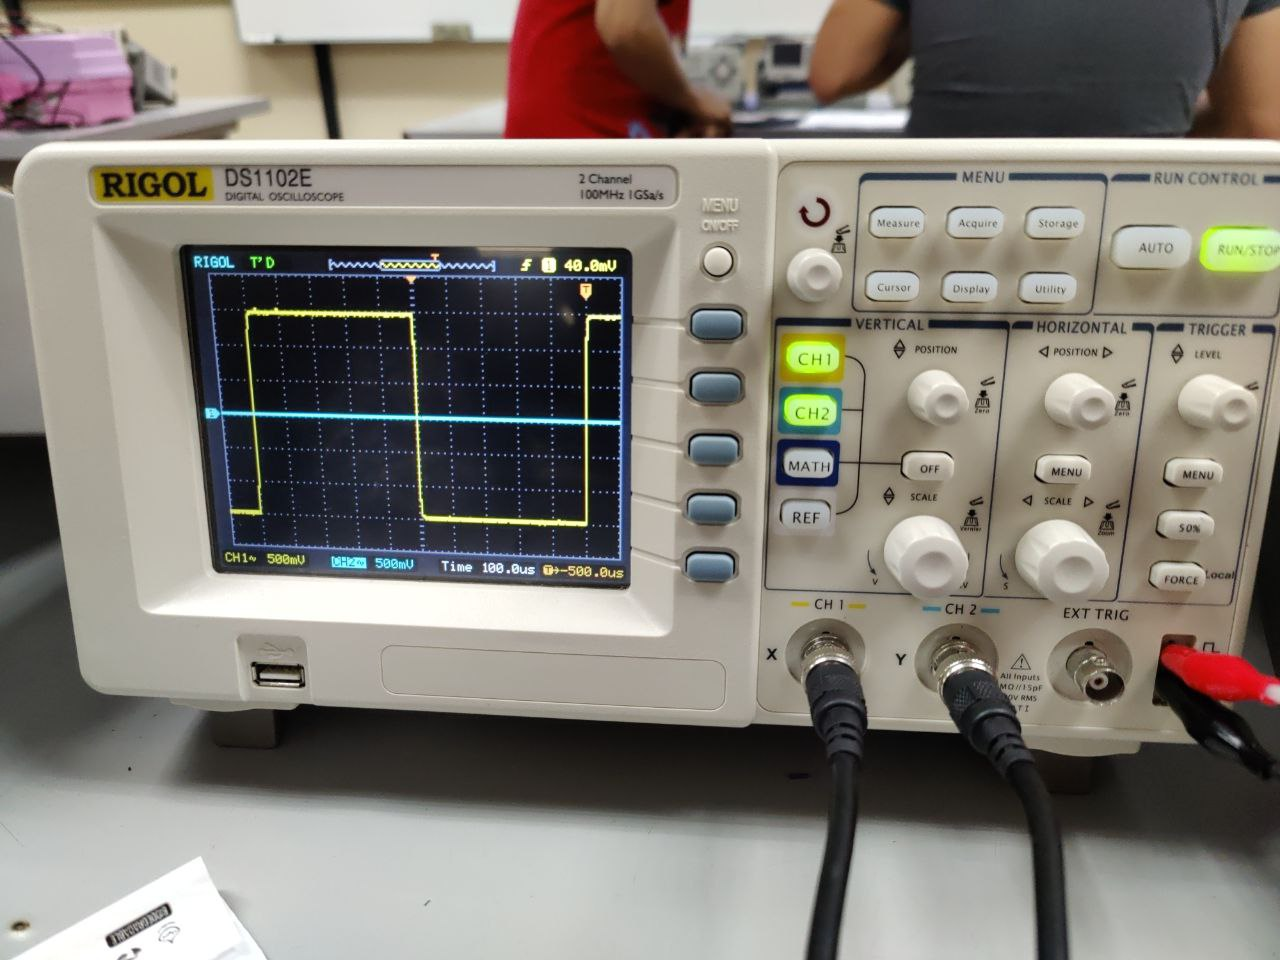
\includegraphics[width=1.2\textwidth]{fig2}
	\end{minipage}
\caption{Conexión del Óhmetro}
\end{figure}

\vspace{.5cm}

\begin{table}[ht!]
\begin{center}
\begin{tabular}{|c c c|}
	\hline
	Resistencia & Medicion con el Óhmetro digital & Valor con el código de colores\\ [0.5ex]
	\hline
	$R_1$ & 585 \si{\ohm} & 560 \si{\ohm}\\
	\hline
	$R_2$ & 1.03k \si{\ohm} & 1k \si{\ohm}\\
	\hline
	$R_3$ & 731 \si{\ohm} & 680 \si{\ohm}\\
	\hline
	$R_4$ & 375 \si{\ohm} & 330 \si{\ohm}\\
	\hline
\end{tabular}
\label{table:1}
\caption{Mediciones de valores resistivos}
\end{center}
\end{table}

\vspace{1cm}

\subsection{Uso del voltímetro}

En la Figura 4 se muestra como se midió el voltaje en un elemento. Se construyo el circuito de la Figura 5. Después se encendió la fuente de voltaje y se obtuvieron los voltajes de la tabla 2.

\begin{figure}[h!]
	\centering
	  \begin{circuitikz}[american, voltage dir=RP]
	  		\draw	(0,0) 
	  		to[battery] (0,3)
			to[short, i=$Carga$] (2,3)
			to[R] (2,0) -- (0,0)	;
			\draw (2,2.5) -- (4,2.5)
			to[voltmeter=Voltímetro] (4,0.5) -- (2,0.5);
		\end{circuitikz}
	\caption{Ejemplo de conexión del voltímetro}
\end{figure}

\vspace{.5cm}

\begin{figure}[!h]
	\centering
	\begin{minipage}{.5\textwidth}
  \centering
	  \begin{circuitikz}[american, voltage dir=RP] 
	  		\draw	(0,0)
	  		to[battery=$E$, name=E] (0,6) -- (3, 6)
	  		to[R=$R_1$ 1k \si{\ohm}] (3,3)
			to[R=$R_2$ 330 \si{\ohm}] (3,0) -- (0,0);
			\ctikztunablearrow{1}{1.2}{-30}{E}
		\end{circuitikz}
	\end{minipage}%
	\begin{minipage}{.5\textwidth}
  \centering
	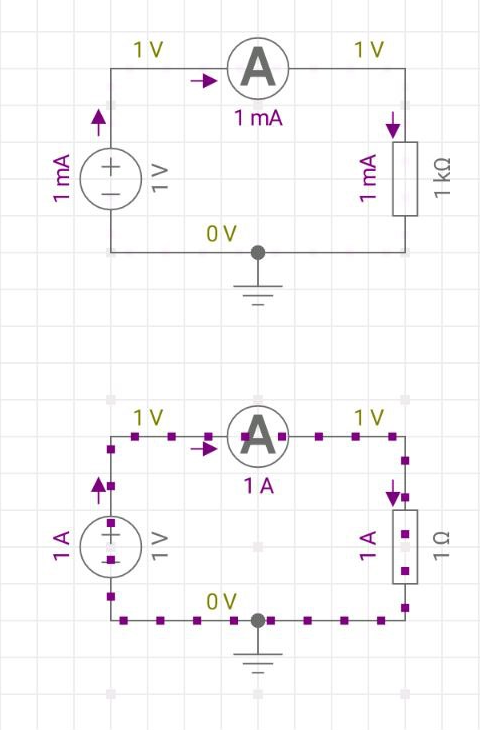
\includegraphics[width=1.3\textwidth]{fig3}
	\end{minipage}
\caption{Circuito en serie}
\end{figure}


\vspace{.5cm}

\begin{table}[ht!]
\begin{center}
\begin{tabular}{|c c c c|}
	\hline
	Voltaje aplicado & Voltaje en $R_1$ y $R_2$ & Voltaje en $R_1$ & Voltaje en $R_2$\\ [0.5ex]
	\hline
	1\si{\volt} & 0.9997\si{\volt} & 0.7455\si{\volt} & 0.25175\si{\volt}\\ \hline
	2\si{\volt} & 1.9967\si{\volt} & 1.4925\si{\volt} & 0.50412\si{\volt}\\ \hline
	3\si{\volt} & 2.9965\si{\volt} & 2.2401\si{\volt} & 0.7567\si{\volt}\\ \hline
	4\si{\volt} & 3.9962\si{\volt} & 2.9869\si{\volt} & 1.0091\si{\volt}\\ \hline
	5\si{\volt} & 4.9990\si{\volt} & 3.7365\si{\volt} & 1.2668\si{\volt}\\ \hline
	6\si{\volt} & 5.9980\si{\volt} & 4.4826\si{\volt} & 1.5151\si{\volt}\\ \hline
	7\si{\volt} & 6.9960\si{\volt} & 5.2284\si{\volt} & 3.7676\si{\volt}\\ \hline
	8\si{\volt} & 7.9968\si{\volt} & 5.9741\si{\volt} & 2.0264\si{\volt}\\ \hline
	9\si{\volt} & 8.9971\si{\volt} & 6.7233\si{\volt} & 2.2744\si{\volt}\\ \hline
	10\si{\volt} & 9.9956\si{\volt} & 7.4688\si{\volt} & 2.5269\si{\volt}\\ \hline
	11\si{\volt} & 10.9964\si{\volt} & 8.2157\si{\volt} & 2.7806\si{\volt}\\ \hline
	12\si{\volt} & 11.9940\si{\volt} & 8.96012\si{\volt} & 3.0347\si{\volt}\\ \hline
\end{tabular}
\label{table:2}
\caption{Mediciones de voltaje}
\end{center}
\end{table}

\vspace{1cm}

\subsection{Uso del amperímetro}

La Figura 6 muestra como conectó el amperímetro para la medición de corriente en un elemento.

\begin{figure}[h!]
	\centering
	  \begin{circuitikz}[american, voltage dir=RP] 
	  		\draw	(0,0) 
	  		to[battery] (0,3)
	  		to[ammeter=Amperímetro, invert] (3,3)
			to[short, i=$Carga$] (3,2)
			to[R] (3,0) -- (0,0);
		\end{circuitikz}
	\caption{Ejemplo de conexión del amperímetro}
\end{figure}


\vspace{.5cm}

\begin{figure}[!h]
	\centering
	\begin{minipage}{.5\textwidth}
	\raggedleft 
	  \begin{circuitikz}[american, voltage dir=RP] 
	  		\draw	(0,0)
	  		to[battery=$E$, name=E] (0,4) -- (1, 4)
	  		to[R=$R_1$ 560\si{\ohm}] (1,0) -- (0,0);
			\draw (1,4) -- (3.5,4)
			to[R=$R_2$ 680\si{\ohm}] (3.5,0) -- (1,0);
			\ctikztunablearrow{1}{1.2}{-30}{E}
		\end{circuitikz}
	\end{minipage}%
	\begin{minipage}{.5\textwidth}
  \centering
	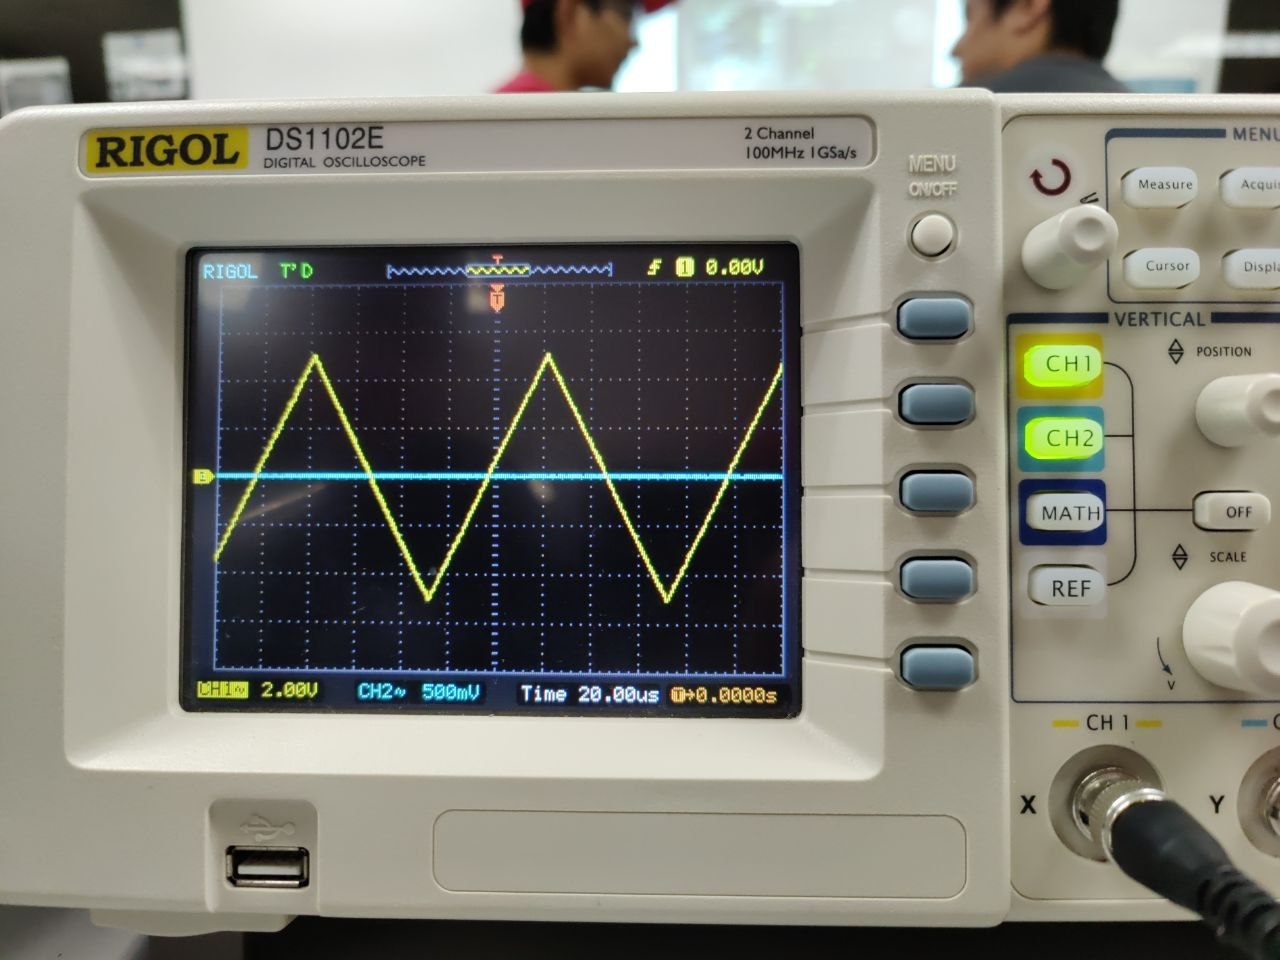
\includegraphics[width=1.3\textwidth]{fig4}
	\end{minipage}
\caption{Circuito en serie}
\end{figure}

Se construyó el circuito de la Figura 7. Después, se encendió la fuente de voltaje y se obtuvieron los valores de la tabla 3.

\vspace{.5cm}

\begin{table}[ht!]
\begin{center}
\begin{tabular}{|c c c c|}
	\hline
	Voltaje aplicado & Corriente en $R_1$ y $R_2$ & Corriente en $R_1$ & Corriente en $R_2$\\ [0.5ex]
	\hline
	1\si{\volt} & 3.149 $m$\si{\ampere} & 1.693 $m$\si{\ampere} & 1.452 $m$\si{\ampere}\\ \hline
	2\si{\volt} & 6.309 $m$\si{\ampere} & 3.380 $m$\si{\ampere} & 2.908 $m$\si{\ampere}\\ \hline
	3\si{\volt} & 9.473 $m$\si{\ampere} & 5.100 $m$\si{\ampere} & 4.365 $m$\si{\ampere}\\ \hline
	4\si{\volt} & 12.640 $m$\si{\ampere} & 6.900 $m$\si{\ampere} & 5.824 $m$\si{\ampere}\\ \hline
	5\si{\volt} & 15.820 $m$\si{\ampere} & 8.770 $m$\si{\ampere} & 7.289 $m$\si{\ampere}\\ \hline
	6\si{\volt} & 19.017 $m$\si{\ampere} & 10.560 $m$\si{\ampere} & 8.750 $m$\si{\ampere}\\ \hline
	7\si{\volt} & 22.609 $m$\si{\ampere} & 12.400 $m$\si{\ampere} & 10.212 $m$\si{\ampere}\\ \hline
	8\si{\volt} & 25.428 $m$\si{\ampere} & 14.255 $m$\si{\ampere} & 11.680 $m$\si{\ampere}\\ \hline
	9\si{\volt} & 28.666 $m$\si{\ampere} & 16.100 $m$\si{\ampere} & 13.160 $m$\si{\ampere}\\ \hline
	10\si{\volt} & 31.830 $m$\si{\ampere} & 17.950 $m$\si{\ampere} & 14.630 $m$\si{\ampere}\\ \hline
	11\si{\volt} & 35.121 $m$\si{\ampere} & 19.800 $m$\si{\ampere} & 16.115 $m$\si{\ampere}\\ \hline
	12\si{\volt} & 38.336 $m$\si{\ampere} & 21.680 $m$\si{\ampere} & 17.600 $m$\si{\ampere}\\ \hline
\end{tabular}
\label{table:3}
\caption{Mediciones de corriente}
\end{center}
\end{table}

\clearpage
\newpage

\section{Cuestionario}

\vspace{.5cm}

\begin{enumerate}
\item ¿Cuál es la característica de un circuito serie?\\
	Dos o más elementos en un circuito se encuentran en serie si la terminal de salida de uno conecta a la terminal de entrada del otro.\par
\item ¿Cuál es la característica de un circuito en paralelo?\\
	Dos o más elementos de un circuito se encuentran en paralelo si sus terminales de entrada se encuentran conectadas al mismo punto, y de forma similar, sus terminales de salida se encuentran conectadas al mismo punto del circuito.\par
\item ¿Cuál es la diferencia principal entre un medidor analógico y un digital?\\
	Los medidores analógicos realizan sus mediciones a través de agujas, mientras que los digitales lo hacen a través de una pantalla y muestran unidades más precisas.\par
\item ¿Por qué un amperímetro no debe conectarse en paralelo?\\
	Una conexión en paralelo distribuye la corriente que pasa antes del punto de conexión en paralelo, por lo cual, la corriente medida sera completa de un lado o parcial de otro.\par
\item ¿Por qué debe des-energizar el circuito cuando se mide la resistencia de un circuito eléctrico?\\
	El Óhmetro cuenta con su propia fuente de alimentación que utiliza para medir la resistencia, por lo que conectarlo a un circuito energizado devolverá una medición errónea.\par
\end{enumerate}

\newpage

\section{Conclusiones}

\vspace{.5cm}

{\Large González Cárdenas Ángel Aquilez}\\
\vspace{.3cm}
En la primer parte de la práctica, se apreció la diferencia entre los valores resistivos que se encontraban señalados por los códigos de colores presentes en cada resistor, y los valores reales que se obtuvieron al utilizar el Óhmetro. Si bien, la mayoría de elementos resistivos se encontró dentro de sus valores esperados (señalados por su nivel de tolerancia), el elemento resistivo de 330 \si{\ohm} presentó un valor que excedió una tolerancia de más del +5\% y +10\%, que se atribuye a un posible daño en las terminales o en su estructura que provocó el aumento de resistencia. En la segunda parte se logró apreciar como se distribuye el voltaje en cada elemento de un circuito en serie, por lo cual es posible decir que la caída de voltaje es mayor si la resistencia del elemento es mayor. Por último, en la tercera parte, se apreció como se distribuye la corriente en un elemento en paralelo, por lo que se concluye que entre menor resistencia tenga un elemento, mayor corriente pasa a través de él.\\

\vspace{.5cm}

{\Large Sánchez González Daniel Iván}\\
\vspace{.3cm}
A la hora de realizar el primer ejercicio de la practica se observó que el valor que el óhmetro daba era aproximadamente el valor esperado, el cual ya se había calculado con anterioridad, sin embargo, la resistencia de 330\si{\ohm} excedido su tolerancia del 5\% lo cual podría ser a causa de un daño en la resistencia.\\
Cuando se midió el voltaje se observó como se distribuye por cada elemento en serie de un circuito, se determino que entre mayor es la resistencia del elemento mayor será el voltaje. Cuando llego la hora de medir la intensidad de corriente en paralelo, en cuyo caso la corriente será mayor cuando hay menor resistencia y viceversa.\\

\section{Anexos}
\subsection{Simulaciones de los circuitos}

A continuación de presentan los resultados de las simulaciones de los circuitos de las figuras 5 y 7 para contrastarlos con las mediciones y cálculos teóricos realizados. Se generaron gracias a la aplicación multiplataforma \textit{EveryCircuit}, presentando los resultados en la Figura 8 para el circuito en serie de la Figura 5, y la Figura 9 para el circuito en paralelo de la Figura 7. Los resultados de las simulaciones se presentan en las respectivas tablas 4 y 5.\\

\begin{figure}[!h]
\centering
	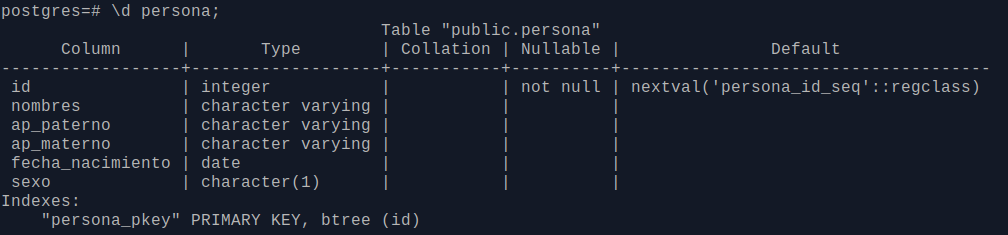
\includegraphics[width=1\textwidth]{fig5}
	\label{fig5}
	 \caption{Simulación del circuito en serie de la Figura 5}
\end{figure}

\begin{table}[ht!]
\begin{center}
\begin{tabular}{|c c c|}
	\hline
	Voltaje aplicado & Voltaje en $R_1$ & Voltaje en $R_2$\\ [0.5ex]
	\hline
	1\si{\volt} & 752m\si{\volt} & 248m\si{\volt}\\ \hline
	2\si{\volt} & 1.5\si{\volt} & 496m\si{\volt}\\ \hline
	3\si{\volt} & 2.26\si{\volt} & 744m\si{\volt}\\ \hline
	4\si{\volt} & 3.01\si{\volt} & 992m\si{\volt}\\ \hline
	5\si{\volt} & 3.76\si{\volt} & 1.24\si{\volt}\\ \hline
	6\si{\volt} & 4.51\si{\volt} & 1.49\si{\volt}\\ \hline
	7\si{\volt} & 5.26\si{\volt} & 1.74\si{\volt}\\ \hline
	8\si{\volt} & 6.02\si{\volt} & 1.98\si{\volt}\\ \hline
	9\si{\volt} & 6.77\si{\volt} & 2.23\si{\volt}\\ \hline
	10\si{\volt} & 7.52\si{\volt} & 2.48\si{\volt}\\ \hline
	11\si{\volt} & 8.27\si{\volt} & 2.73\si{\volt}\\ \hline
	12\si{\volt} & 9.02\si{\volt} & 2.98\si{\volt}\\ \hline
\end{tabular}
\label{table:2}
\caption{Resultados de la simulación para el voltaje}
\end{center}
\end{table}

\vspace{1cm}

\begin{figure}[!h]
\centering
	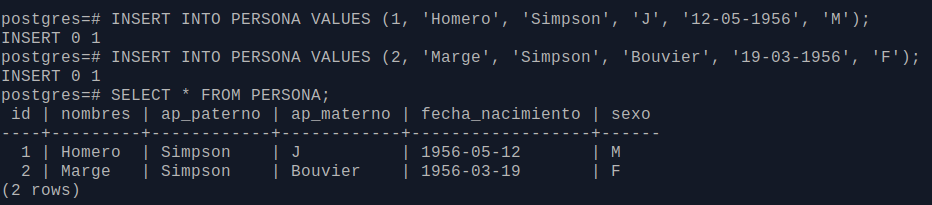
\includegraphics[width=1.1\textwidth]{fig6}
	\label{fig5}
	 \caption{Simulación del circuito en paralelo de la Figura 7}
\end{figure}

\begin{table}[ht!]
\begin{center}
\begin{tabular}{|c c c c|}
	\hline
	Voltaje aplicado & Corriente en $R_1$ y $R_2$ & Corriente en $R_1$ & Corriente en $R_2$\\ [0.5ex]
	\hline
	1\si{\volt} & 3.26 $m$\si{\ampere} & 1.79 $m$\si{\ampere} & 1.47 $m$\si{\ampere}\\ \hline
	2\si{\volt} & 6.51 $m$\si{\ampere} & 3.57 $m$\si{\ampere} & 2.94 $m$\si{\ampere}\\ \hline
	3\si{\volt} & 9.77 $m$\si{\ampere} & 5.36 $m$\si{\ampere} & 4.41 $m$\si{\ampere}\\ \hline
	4\si{\volt} & 13 $m$\si{\ampere} & 7.14 $m$\si{\ampere} & 5.88 $m$\si{\ampere}\\ \hline
	5\si{\volt} & 15.2 $m$\si{\ampere} & 8.93 $m$\si{\ampere} & 6.25 $m$\si{\ampere}\\ \hline
	6\si{\volt} & 19.5 $m$\si{\ampere} & 10.7 $m$\si{\ampere} & 8.82 $m$\si{\ampere}\\ \hline
	7\si{\volt} & 22. $m$\si{\ampere} & 12.5 $m$\si{\ampere} & 10.3 $m$\si{\ampere}\\ \hline
	8\si{\volt} & 26.1 $m$\si{\ampere} & 14.3 $m$\si{\ampere} & 11.8 $m$\si{\ampere}\\ \hline
	9\si{\volt} & 29.3 $m$\si{\ampere} & 16.1 $m$\si{\ampere} & 13.2 $m$\si{\ampere}\\ \hline
	10\si{\volt} & 32.6 $m$\si{\ampere} & 17.9 $m$\si{\ampere} & 14.7 $m$\si{\ampere}\\ \hline
	11\si{\volt} & 35.8 $m$\si{\ampere} & 19.6 $m$\si{\ampere} & 16.2 $m$\si{\ampere}\\ \hline
	12\si{\volt} & 39.1 $m$\si{\ampere} & 21.4 $m$\si{\ampere} & 17.6 $m$\si{\ampere}\\ \hline
\end{tabular}
\label{table:3}
\caption{Resultados de la simulación para la corriente}
\end{center}
\end{table}


\end{document}